\section*{Dynamic Programming}
The following example will use the Fibonnaci sequence 
\begin{align*}
    F(n) = 
    \begin{cases}
        1 & \text{ if } n \leq 2 \\
        F(n-1) + F(n-2) &\text{ if } n > 2
    \end{cases}
\end{align*} 

\begin{enumerate}
    \item Recursion
        \begin{itemize}[leftmargin = 1em]
            \item is pretty shit in terms of run time
        \end{itemize}
    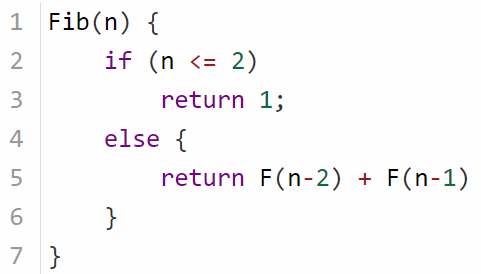
\includegraphics[scale = 0.6]{pictures/fibonacci recursion.png}
    \item Top-down Memoization
    \begin{itemize}[leftmargin = 1em]
        \item store past calls/results to memory
        \item needs helper $\rightarrow$ in helper check if it's been computed yet, usually means checking if the entry is 0 or $-1$
    \end{itemize}
    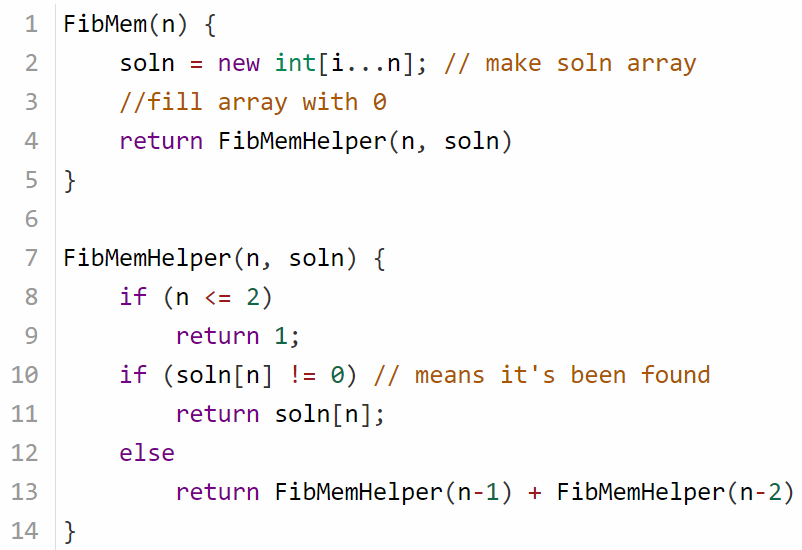
\includegraphics[scale = 0.6]{pictures/fibonacci memoized.png}
    \item Dynamic Programming (Bottom-Up)
        \begin{itemize}[leftmargin = 1em]
            \item calculate all necessary entries first
            \item use for loop $\rightarrow$ usually code inside for loop is direct translation of recurrence relation
        \end{itemize}
    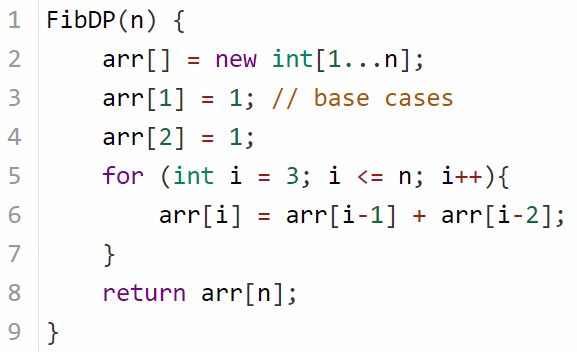
\includegraphics[scale = 0.6]{pictures/fibonacci dp.png}
\end{enumerate}
\begin{itemize}
    \item making change problem: give the minimum number of change for a dollar amount - imagine all possible coins are \$0.25, \$0.10, and \$0.01. 
\end{itemize} 
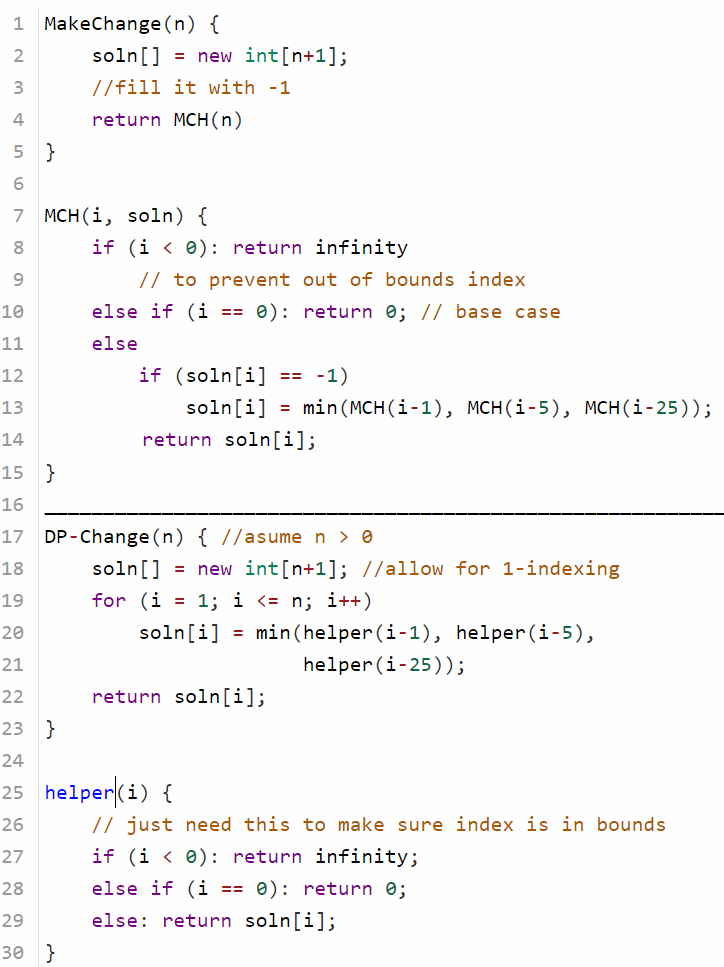
\includegraphics[scale = 0.7]{pictures/Change code.png} 
\begin{itemize}
    \item \ul{\textbf{runtime}}
    \begin{itemize}[leftmargin = 1em]
        \item recursion: see how many recursive call is called per iteration (call $a$), and how deep the recursive call (call $b$) - get $a^b$, multiply that with time for the base case
        \begin{itemize}[leftmargin = 1em]
            \item ex. Fibonacci: 2 recursive call, each getting called n times $r\rightarrow 2^n$ factor and base case is $O(1)$ - so total runtime is $O(2^n)$
        \end{itemize}
    
        \item Memoization \& DP: think about how much work you're doing without recursive call and then think about how many (non-repetitive) recursive call you're making, then calculate the total 
        \begin{itemize}[leftmargin = 1em]
            \item thinking about it in terms of for loops and DP makes a bit more sense
            \item ex. Fibonacci: Work without recursive call is $\Theta(1)$. Number of unique recursive call is $\Theta(n)$. So total is $\Theta(n)$ 
        \end{itemize}
    \end{itemize}
    \vfill \null \columnbreak
    \item tips - when identifying sub problems
    \begin{itemize}[leftmargin = 1em]
        \item if problem involve discrete quantities then sub problem would be about smaller quantities $\rightarrow$ going backwards - likely memoization
        \item if problem is going forward (computing the next value or seeing if going forward in 1 direction gives the max/min - i.e midterm scheduling q) $\rightarrow$ likely DP
    \end{itemize}
\end{itemize}

